\documentclass{article}
\usepackage{amsmath}
\usepackage{amsfonts}
\usepackage{graphicx}
\usepackage{listings}


\title{Cut-Based Least-Squares Spectral Analysis}
\author{M.P.Ross based on work by the E\"ot-Wash group}

\begin{document}
\maketitle

\section{Least-Squares Fitting}

Let's say we have data from an instrument, $y_i$, that are independent from each other and who's errors are Gaussian.
\begin{equation}
y\sim y(t)+N(0, \sigma_y)
\end{equation}

And let's say we want to fit this to a discrete set of frequencies. Here we will focus on just two frequencies but this can be readily generalized to as many frequencies as one wants. The model we will fit to is:
\begin{equation}
\hat{y}= a_1 \cos(\omega_1 t)+b_1 \sin(\omega_1 t)+a_2 \cos(\omega_2 t)+b_2 \sin(\omega_2 t)
\end{equation}

This can be recast into vector notation as:

\begin{equation}
\hat{y}= \mathbf{X} \beta
\end{equation}
with
\begin{equation}
\beta = [a_1, b_1, a_2, b_2]^T
\end{equation}
\begin{equation}
\mathbf{X}= [\cos(\omega_1 t), \sin(\omega_1 t), \cos(\omega_2 t), \sin(\omega_2 t)]^T
\end{equation}

We call the columns of $\mathbf{X}$ the basis functions. In general these could be any set of functions but here we're focusing on just sinusoidal functions. Say we have a number of data points, $n$, of $y_i$ at given $t$. Then 
\begin{equation}
y=n\times 1
\end{equation}
\begin{equation}
\beta=4 \times 1
\end{equation}
\begin{equation}
\mathbf{X}=n \times 4
\end{equation}

Using linear-least squares fitting, we minimize the residual sum-of-squares, $R$,with respect to $\beta$ :
\begin{equation}
R=(y- \mathbf{X} \beta)^2
\end{equation}
\begin{equation}
R=(y- \mathbf{X} \beta)^T(y- \mathbf{X} \beta)
\end{equation}

At the minimum:
\begin{equation}
\frac{\partial R}{\partial \beta}=0
\end{equation}

Evaluating the derivative given us:
\begin{equation}
0=-2 \mathbf{X}^T(y- \mathbf{X} \beta)
\end{equation}

Rearranging:
\begin{equation}
\beta=(\mathbf{X}^T\mathbf{X})^{-1}\mathbf{X}^T y\label{fit}
\end{equation}

At the end this allows one to construct $\mathbf{X}$ for the frequencies of interest and quickly fit the data with a simply one line matrix multiplication. The parameters that come out also need no corrections and can easily be shifted into amplitude and phase using (for $\omega_1$):
\begin{equation}
A_1=\sqrt{\beta_1^2+\beta_2^2}
\end{equation}
\begin{equation}
\phi_1=\arctan(\beta_2/\beta_1)
\end{equation}


\section{Orthogonality}
In order to prevent spectral leakage (power from one frequency going to the other), the basis functions must be orthogonal. Orthogonality also makes the error analysis and interpretation more straight forward. For the basis functions to be orthogonal then:
\begin{equation}
(\mathbf{X}^T\mathbf{X})_{ij} \propto \delta_{ij}
\end{equation}

With $\mathbf{X}= [\cos(\omega_1 t), \sin(\omega_1 t), \cos(\omega_2 t), \sin(\omega_2 t)]^T$, this can be satisfied with two conditions. $\mathbf{X}^T\mathbf{X}$ has the following form:

\[
\mathbf{X}^T\mathbf{X} =\begin{bmatrix}
    \sum \cos^2(\omega_1 t)      &  \sum \cos(\omega_1 t)\sin(\omega_1 t)& \sum \cos(\omega_1 t)\cos(\omega_2 t)& \sum \cos(\omega_1 t)\sin(\omega_2 t) \\
    \\
   \sum \sin(\omega_1 t)  \cos(\omega_1 t) &  \sum \sin^2(\omega_1 t)  & \vdots & \vdots\\
   \\
     \sum \cos(\omega_2 t) \cos(\omega_1 t)   &   \dots &  \sum \cos^2(\omega_2 t)  & \vdots\\
     \\
    \sum\sin(\omega_2 t)  \cos(\omega_1 t)  &   \hdots& \hdots&  \sum \sin^2(\omega_2 t)  
\end{bmatrix}
\]
\\

Where the sums are from $t=0$ to some undetermined length, $T$. In order to make 
\begin{equation}
\sum_{t=0}^T \cos(\omega_1 t)\sin(\omega_1 t)=0
\end{equation}

Then $T=2\pi m/\omega_1$ where $m\in \mathbb{Z}^+$. This same argument follows for the $\omega_2$ entries so the length of the data must be an integer multiple of both periods in question. 

With the first condition met, then $\omega_1 \neq \omega_2$ ensures that
\begin{equation}
\sum_{t=0}^T \cos(\omega_1 t)\cos(\omega_2 t)=0
\end{equation}

With both of these conditions met then 
\begin{equation}
\sum_{t=0}^T \cos^2(\omega_1 t)=\frac{m}{2}
\end{equation}

Thus,
\begin{equation}
\mathbf{X}^T\mathbf{X} =\frac{m}{2} \delta_{ij}
\end{equation}

So as long as we don't try to fit to the same frequency, we can pick the length of data to fit to ensure orthogonality. Then each parameter of the fit is independent from the others and both the interpretation and the error analysis is much easier. 

\section{Error Analysis}

In almost every circumstance, we also need to be able to derive an uncertainty on our fit parameters. Linear-least squares again comes to our rescue.

Let assume that there are no errors in the measurement of $t$ (and therefore $\sigma_X=0$) and that the data points of $y$ are independent with errors drawn from a normal distribution, $N(0,\sigma_y)$. 

It can be shown that with the above conditions, $\beta$ is also described by a normal distribution with a standard deviation of:

\begin{equation}
\sigma_\beta^2=(\mathbf{X}^T\mathbf{X})^{-1} \sigma_y^2
\end{equation}

If the data points of $y$ are not independent (equivalent to $y$ not having a white noise spectrum) then one can generalized least squares to account for the covariance between $y$-data points.

\section{Cut-Based Analysis}

Real instrumentation is not as simple as the model that we have been using, apparatus get bumped, earthquakes happen, and electronics glitches. To get around this we can break the data in question into ``cuts'' and disregard those that have these disturbances. Figure \ref{raw} shows simulated data of a sinusoidal signal with Gaussian noise and random ``glitches''.  Here we will focus on extracting amplitudes from just a single sinusoidal signal since visualizing a two parameter fit is much easier than four or more parameters. 


\begin{figure}[!h]
\begin{centering}
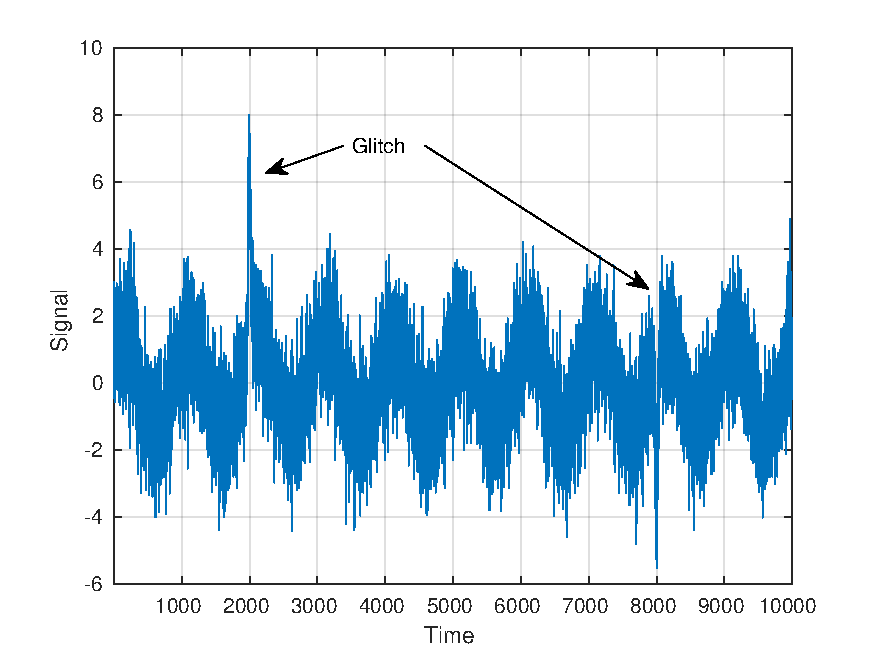
\includegraphics[width=\textwidth]{RawData.pdf}
\caption{Simulated data with glitches and sinusoidal signal we want to extract.}\label{raw}
\end{centering}
\end{figure}

In order to avoid having the results skewed by these disturbances, we can break the data into ``cuts'' of a set length and toss out the cuts which contain glitches. The length of these cuts needs to be chosen to satisfy the orthogonality conditions discussed above. Additionally, we want to keep the $m$ low (usually 1 or 2) so that we toss out the least amount of data.

Once we've broken the data into these cuts, we fit each one using Equation~\ref{fit} as well as calculate the misfit-squared (chi-squared) defined as:

\begin{equation}
\chi^2=\sum (y-\mathbf{X}\beta)^2
\end{equation}

This statistic tells us how much the data follows the model with the fit parameters. When we look at the distribution of this, shown in Figure \ref{cut}, we can see that most of the cuts are clustered around one value while a collection are much higher. These higher values indicate that those cuts have a disturbance within them. 

To toss these out we set a misfit-squared threshold that keeps the good data points while tossing out the bad. This threshold is somewhat subjective so the effects of one's choice must be studied to ensure a non-biased result. 

\begin{figure}[!h]
\begin{centering}
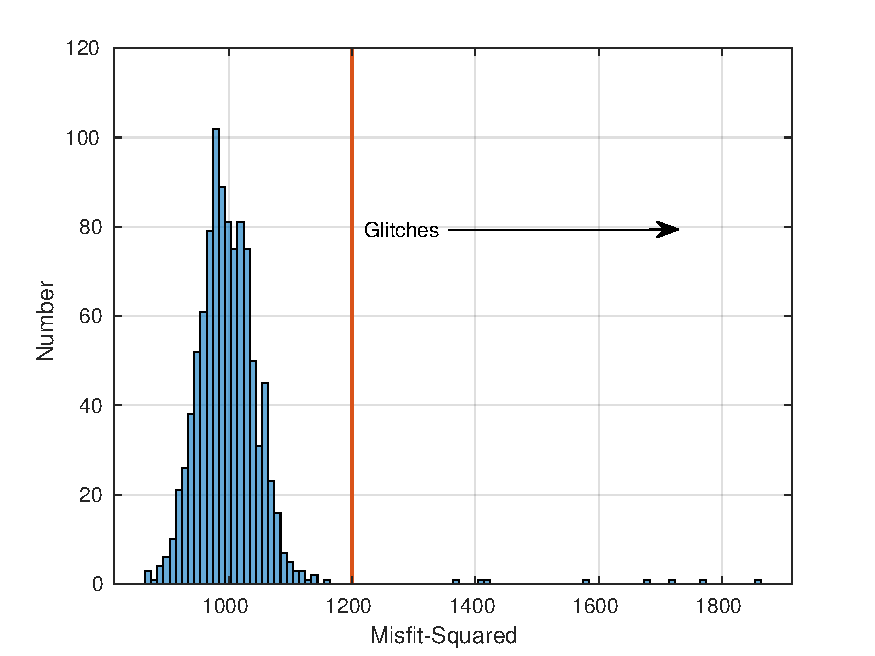
\includegraphics[width=\textwidth]{MisfitCut.pdf}
\caption{Misfit-squared distribution along with cut threshold shown in red.}\label{cut}
\end{centering}
\end{figure}

\pagebreak

The effects of this cut on the distribution of fit parameters can be seen in Figure \ref{dist} which shows the sine and cosine fit amplitudes for the data shown in Figure \ref{raw}. Before the cut there are a number of outliers which would skew the means of the amplitudes and expand the uncertainties. The cut removes these and what's left over is a Gaussian distribution of points with a mean at the correct value.

An additional utility of this method is that we can analyze the distribution of the fit parameters to extract an uncertainty without knowledge of the errors of the data points. Although we know that if the input data has Gaussian errors then the fit parameters will also be Gaussian, if we don't know the input data errors we don't know a priori what the errors on the fit parameters will be. The cut based analysis allows us to directly observe the distribution of these errors since we are effectively resampling the underlying distribution with each cut (after the glitch removal that is). 


\pagebreak

\begin{figure}[!h]
\begin{centering}
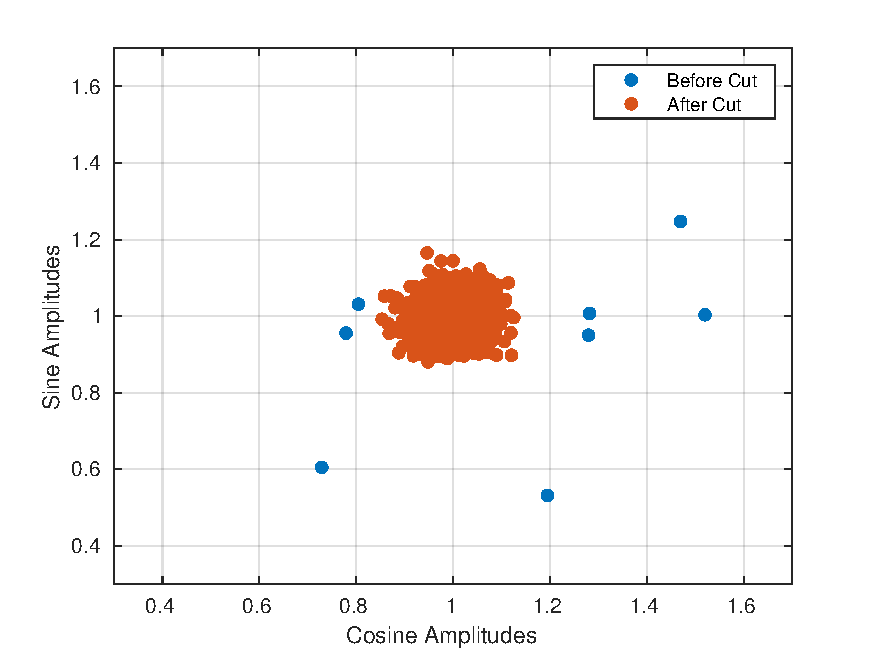
\includegraphics[width=\textwidth]{FitDist.pdf}
\caption{Cosine and sine fit amplitude before and after the misfit-squared cut.}\label{dist}
\end{centering}
\end{figure}

If the fit parameter distribution follows a Gaussian then we can use standard equations to extract the mean and the standard deviation of the mean:

\begin{equation}
\mu =\frac{1}{N} \sum a_i
\end{equation}
 
\begin{equation}
\sigma^2_\mu= \frac{\sigma_a^2 }{N}
\end{equation}

The uncertainty of the measurement then follows $1/\sqrt{\text{periods}}$ as long as the instrument stays constant throughout the measurement. This is a very generic result and is also the case in standard Fourier analysis methods. This can be seen in Figure \ref{err} where it is evident that the error falls off as expected.

This has the important consequence that there are two ways of decreasing the error on a measurement. One is to make the error on the input data, $\sigma_y$, smaller which in turn makes the error on the fit parameter, $\sigma_\beta$ smaller. The other is to measure the signal for longer. This is analogous to integrating a coherent signal in a standard Fourier analysis. However, the relative gain from this second method shrinks with time so for real systems that can't be observed for infinite time, this method can only get you so far. For example Figure \ref{err} shows that for the simulation we can decrease the errors by a factor of $\sim5$ after 400 periods but only decrease it another $\sim25\%$ in the following 600 periods.

\begin{figure}[!h]
\begin{centering}
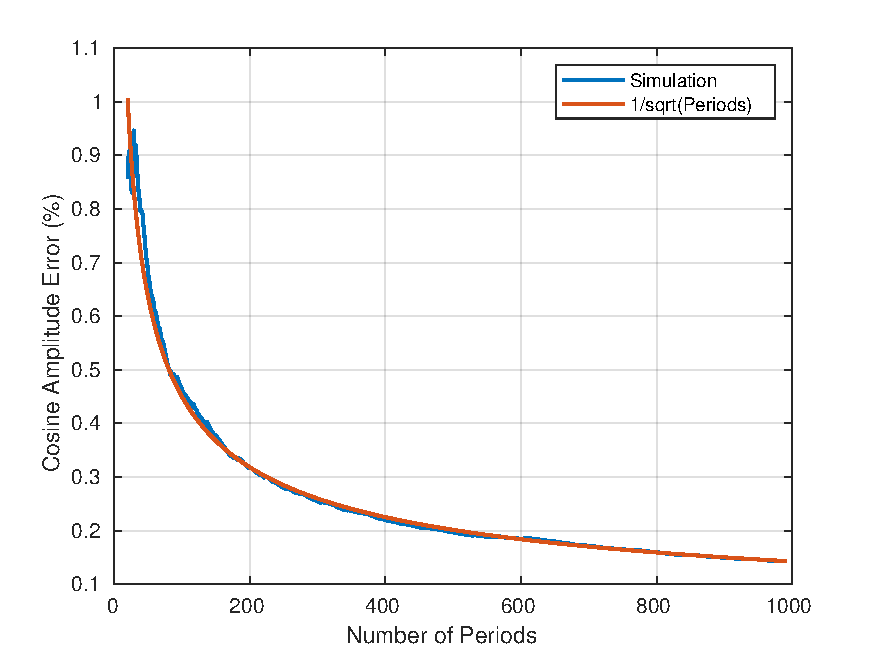
\includegraphics[width=\textwidth]{ErrorVsPeriods.pdf}
\caption{Percentage error for the cosine amplitude as a function of number of periods observed.}\label{err}
\end{centering}
\end{figure}
\pagebreak
\section{Simulation Code}

\begin{lstlisting}
%% Data creation
f=1/1000;

in=[];
out=[];
chi=[];
timStamp=[];

n=1e6

tim=linspace(1,n,n);
sig=cos(2*pi*f*tim)+sin(2*pi*f*tim)+randn(1,n)...
    +5*gaussmf(tim,[20 randn*n/2])-5*gaussmf(tim,[20 randn*n/2])...
    +5*gaussmf(tim,[20 randn*n/2])-5*gaussmf(tim,[20 randn*n/2])...
    +5*gaussmf(tim,[20 randn*n/2])-5*gaussmf(tim,[20 randn*n/2])...
    +5*gaussmf(tim,[20 randn*n/2])-5*gaussmf(tim,[20 randn*n/2])...
    +5*gaussmf(tim,[20 2000])-5*gaussmf(tim,[20 8000]);


%% Fitting
periods=1;

for index=1:n*f/periods-1
        timCut=tim(periods*index/f:periods*(index+1)/f);
        sigCut=sig(periods*index/f:periods*(index+1)/f);

        x=[cos(2*pi*f*timCut); sin(2*pi*f*timCut)];

        w=inv(x*x')*x*sigCut';

        in=[in; w(1)];
        out=[out; w(2)];

        mis=[mis; sum((sigCut'-x'*w).^2)];

end

%% Misfit-Squared Cut
misLim=1200

index=find(mis<misLim);
inCut=in(index);
outCut=out(index);
misCut=mis(index);

%% Averaging
avg=[];
err=[];
nPoints=[];

for index=20:length(inCut)
    cut=inCut(1:index);
    avg=[avg; mean(cut)];
    err=[err; std(cut)/sqrt(length(cut))];
    nPoints=[nPoints; index];
end

\end{lstlisting}

\end{document}